\section{Sea Battle 2}

\begin{figure}
    \centering
    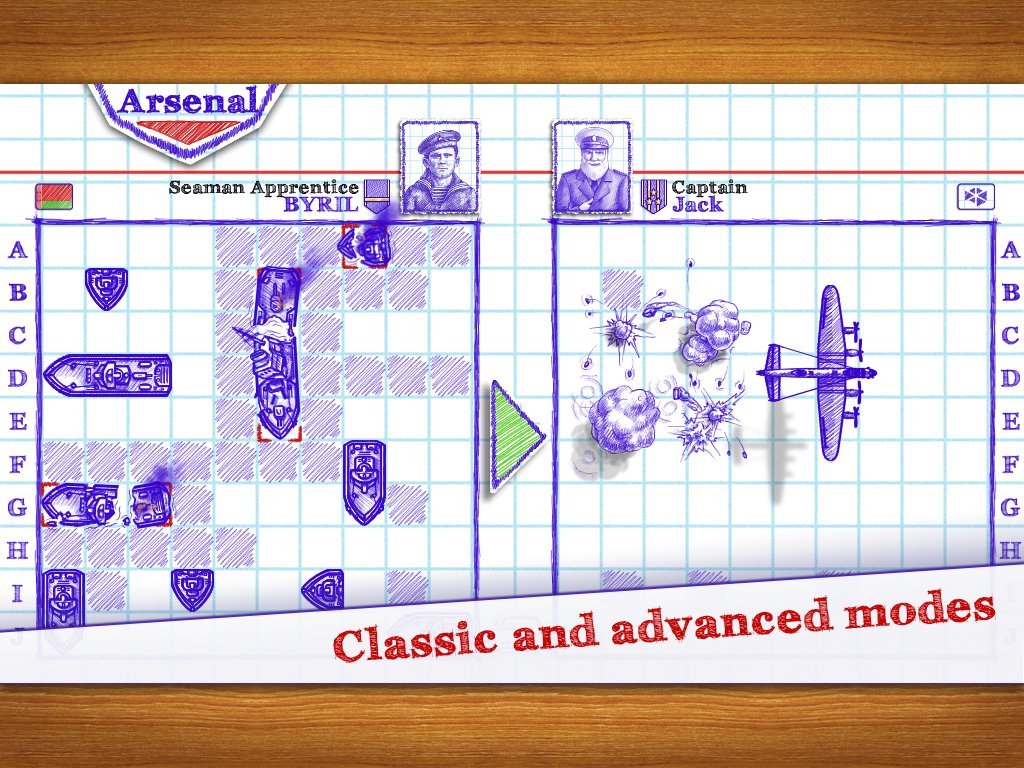
\includegraphics[width=0.5\linewidth]{assets/competitive-apps/sea-battle.jpg}
    \caption{Screenshot hry Sea Battle 2~\cite{byril_sea_battle_2}}
    \label{fig:sea-battle}
\end{figure}

Hra \emph{Sea Battle 2} sice není postavena na kooperaci a komunikaci mezi
hráči,
ale představuje hezkou reprezentaci klasické stolní hry v moderním pojetí.
Hráči z celého světa mezi sebou na svých zařízeních vedou souboje
a za každé vítězství postupně postupují v námořních
hodnostech.~\cite{byril_sea_battle_2}

Herní plocha obsahuje $10 \times 10$ políček,
kam si hráč rozloží své lodě.
Vedle toho jsou postupně vyobrazovány políčka protihráče.
UI je lazeno do podoby čtverečkovaného papíru s ručně kreslenými prvky.

Cílem hry, stejně jako v klasické stolní hře,
je zneškodnit všechny protivníkovy lodě.
Toho lze docílit klasicky pomocí bombardování,
nebo v pokročilém módu pomocí nejrůznějších letadel a pokročilých děl.
Pokročilý mód hezky rozšiřuje hru o nové strategie,
čímž činí hru zajímavější.

\subsection*{Klady}

\begin{itemize}
    \item Známý koncept hry.
    \item Obohacení hry s pokročilým módem o nové prvky.
\end{itemize}

\subsection*{Zápory}

\begin{itemize}
    \item UI nepůsobí přívětivě.
    \item UI nelze přibližovat,
    což způsobuje problémy s dotyky na jednotlivá políčka.
\end{itemize}
